%%%% ijcai19.tex

\typeout{IJCAI-19 Instructions for Authors}

% These are the instructions for authors for IJCAI-19.

\documentclass{article}
\pdfpagewidth=8.5in
\pdfpageheight=11in
% The file ijcai19.sty is NOT the same than previous years'
\usepackage{ijcai19}

% Use the postscript times font!
\usepackage{times}
\usepackage{soul}
\usepackage{url}
\usepackage[hidelinks]{hyperref}
\usepackage[utf8]{inputenc}
\usepackage[small]{caption}
\usepackage{graphicx}
\usepackage{subfigure}
\usepackage{amsmath}
\usepackage{booktabs}
\usepackage{algorithm}
\usepackage{algorithmic}
\usepackage{multirow}
\usepackage{array}
\urlstyle{same}
% the following package is optional:
%\usepackage{latexsym} 

% Following comment is from ijcai97-submit.tex:
% The preparation of these files was supported by Schlumberger Palo Alto
% Research, AT\&T Bell Laboratories, and Morgan Kaufmann Publishers.
% Shirley Jowell, of Morgan Kaufmann Publishers, and Peter F.
% Patel-Schneider, of AT\&T Bell Laboratories collaborated on their
% preparation.

% These instructions can be modified and used in other conferences as long
% as credit to the authors and supporting agencies is retained, this notice
% is not changed, and further modification or reuse is not restricted.
% Neither Shirley Jowell nor Peter F. Patel-Schneider can be listed as
% contacts for providing assistance without their prior permission.

% To use for other conferences, change references to files and the
% conference appropriate and use other authors, contacts, publishers, and
% organizations.
% Also change the deadline and address for returning papers and the length and
% page charge instructions.
% Put where the files are available in the appropriate places.

% \title{Social Relationship Detection using Rules}

\title{Understanding social relationship with person-pair relations}

% Single author syntax
\author{
    Sarit Kraus
    \affiliations
    Department of Computer Science, Bar-Ilan University, Israel \emails
    pcchair@ijcai19.org
}

% Multiple author syntax (remove the single-author syntax above and the \iffalse ... \fi here)
% Check the ijcai19-multiauthor.tex file for detailed instructions
\iffalse
\author{
First Author$^1$
\and
Second Author$^2$\and
Third Author$^{2,3}$\And
Fourth Author$^4$
\affiliations
$^1$First Affiliation\\
$^2$Second Affiliation\\
$^3$Third Affiliation\\
$^4$Fourth Affiliation
\emails
\{first, second\}@example.com,
third@other.example.com,
fourth@example.com
}
\fi

\begin{document}

\maketitle

\begin{abstract}
% Social relationships play a very important role in social network. Social relationship understanding has attracted increasing attention, typically, which can help to understand the behavior of humen in our daily life. Previous social relationship understanding models focused too much on relationships between the same pair and ignore the interplay of different relationships in the same scene.  We found that the interaction between the relationships in the same scene plays an important role in the understanding of social relations and we can make meanful use of rules during inference. This paper proposes a novel model named {\it SRDR} which incorporates rules seamlessly into the deep learning model named {\it SR}  to solve the social relationship understanding problem. It formulates inference as an integer linear programming (ILP) problem, with the objective function generated from {\it SR} and the constraints translated from rules. By incorporating rules, our approach can greatly reduce the solution space and significantly improve the inference accuracy of social relationship understanding models. Experimental results on two classic data sets show that our approach significantly outperforms state-of-the-art  models in social relationship understanding, which justifies the significance of incorporating rules seamlessly into the deep learning model in social relationship understanding task.

Social relationships understanding is to infer the social relations among people from images and videos, which has attracted increasing attention in computer vison recently. A great progress has been made since the rise of deep learning. However, they mostly focuses on the facial attributes or contextual object cues without taking into account the interaction among person pairs. Motivated by scene graph generation, we carefully analyzed the datasets and found the social relations in a still image always have high semantic relevance. For instance, if two person pair in an image are {\it Friends}, then the third one is always friends or at least other intimate relations but not {\it No Relation}. Therefore, to capture this interaction cues, we propose a novel end-to-end trainable Person-Pair Relation Network (PRN) using standard RNNs, a graph inference network that learns iteratively to improve its predictions via message passing among person pair nodes. Extensive experiments on PISC and PIPA-Relation show the superiority of our method over previous methods. 

\end{abstract}

\section{Introduction}
Social relationships are closely related to our daily life \cite{DBLP:conf/wacv/BarrCBF14}. After understanding the social relationship between the person pair, we can easily explain their behavior. For machines, only when they fully understand the social relationships, can they further understand and infer the human behavior in our social life, so as to make a better response. In addition, we often leave traces that capture social relationships in many medias and we not only want the machines to be proficient at their task, but also enable them to blend in and
act appropriately in different situations \cite{DBLP:conf/cvpr/SunSF17}. In short, social relationship detection task is very significant in many ways. In our work, we aim to address the social relationship detection task for every picture where each picture represents a scene. 

However, to solve the social relationship detection task is not so simple. For a giving picture, detecting the social relationships of all the person pair is a difficult task. The models need to be adapted to different scenes and context information to make right judgments.  \cite{DBLP:conf/cvpr/SunSF17} use the information of head region, body region and human attributes to predict the person-pair's social relationship separately. \cite{DBLP:conf/iccv/LiWZK17} make use of the pair of people in question and region proposals and allocate attention to each region to detect the social relationship of each person pair. \cite{DBLP:conf/ijcai/WangCRYCL18} takes advantage of the message propagation between person pair social relationship and the object  semantic regions to solve the problem. The biggest problem of these models is that they all only detect one relationship per step which will cause that different social relationships in the same scene cannot interact with each other. Social relationships in the same scene are strongly linked but the previous models have ignored this important information.

[Figure 1]

As one example in PIPA(Figure 1) where the picture denotes a scene. There are "father-child" relationship, "mother-child" relationship, "grandpa-grandchild" relationship and "grandma-grandchild" relationship in the scene. We can easily see that these relationships are related and belong to the "Attachment" relationship. In other words, we can easily use the interaction of different relationships in the same scene to detect each social relationship. Therefore we address the issue with focusing more on the interaction between every social relationships in one scene to improve the detection performance.

However, the biggest issue of the task is that it is not as simple as people directly judging the result. We need to design the mechanism of the interaction between social relationships and effectively model the mechanism. The other issue is how to use less effective information to model the interaction machanism and get the better result.

To address this problem, we propose a novel end-to-end trainable Person-Pair Relation Network (PRN).

\section{Related Work}

This part will be written by {\bf liangjinrui} and it will be surveyed by {\bf liangjinrui} and {\bf chenhaicheng} by January 31.

\subsection{Social Relationship Understanding}
% Introduce social relationship understanding including \cite{DBLP:conf/aaai/GuoWWWG18}, \cite{DBLP:conf/iccv/LiWZK17}, \cite{DBLP:conf/ijcai/WangWG15} and \cite{DBLP:conf/ijcai/WangCRYCL18}.

The foundation of social network is the social relationships understanding, an important multidisciplinary problem that has attracted increasing attention in computer vision recently. A much number of studies that aim to infer social relationships from images \cite{DBLP:conf/ijcai/WangWG15,DBLP:conf/iccv/LiWZK17,DBLP:conf/ijcai/WangCRYCL18,DBLP:conf/eccv/WangGLF10,DBLP:conf/iccv/ZhangLLT15} and videos \cite{DBLP:conf/eccv/DingY10,DBLP:conf/cvpr/RamanathanY013,DBLP:journals/ivc/VinciarelliPB09} have been made since the rise of deep learning. For instance, motivated by psychological sudies, \cite{DBLP:conf/iccv/ZhangLLT15} and \cite{DBLP:conf/iccv/DibekliogluSG13} exploit social relationships based on facial attributs such as expression and head pose, and affective behaviour analysis. Besides, \cite{DBLP:conf/iccv/LiWZK17} and \cite{DBLP:conf/ijcai/WangCRYCL18} discover that contextual cues around people play a significant role in social realtionship infering. Concretely, \cite{DBLP:conf/iccv/LiWZK17} proposed a dual-glance model for social relationship, where the first glance makes a coarse relationship prediction for a given person pair and then the second one refines the prediction by using the objects around the pair. \cite{DBLP:conf/ijcai/WangCRYCL18} constructed a semantic-aware knowledge graph and employed Gated Graph Neural Network (GGNN) \cite{DBLP:journals/tomccap/LiSKJZW15} to integrate the graph into the Graph Reasoning Model (GRM), a graph reasoning network where a proper message propagation and graph attention mechanism are introduced to explore the interaction between person pair and the contextual objects. \\
Unlike the aforementioned works which mainly focus on facial attributs or contextual object cues, we detaily studied the two classic datasets PISC \cite{DBLP:conf/iccv/LiWZK17} and PIPA-relation \cite{DBLP:conf/cvpr/SunSF17} and found the social relations in a still image have high semantic relevance. Based on this discovery, we designed a novel end-to-end trainable Person-Pair Relation Network (PRN), a graph inference network to capture this semantic relevance cues via message passing among person pair nodes.

\subsection{Message Passing}%


Introduction to Message Passing, written by {\bf liangjinrui}.
 


\subsection{Rules and ILP}

Introduce rules and ILP referring to \cite{DBLP:conf/ijcai/WangWG15}



\section{PRN model}
This part will be written by {\bf liangjinrui} and {\bf chenhaicheng}.
{\bf [model figure]}

[Introduce the total model]

\subsection{Social Relationship Understanding Model}
\subsection{Imposing Rules}
\subsection{Integrating by Integer Linear Programming}


\section{Experiments}

This part will be written by {\bf chenhaicheng}.
\subsection{Experiment Setting}

{\bf Datasets.} In this work, two datasets were used to evaluate our proposed method and other existing ones. The first one is the large-scale People in Social Context (PISC) \cite{DBLP:conf/iccv/LiWZK17} with 22,670 images and contains two-level recognition tasks: {\bf 3 Coarse-level relationship}, namely {\it No Relation, Intimate Relation, None-Intimate Relation} and {\bf 6 Fine-level relationship}, i.e., {\it Friend, Family, Couple, Professional, Commerical, No Relation}. The second one is the People in Photo Album Relation (PIPA-Relation) \cite{DBLP:conf/cvpr/SunSF17}, an extension verson of People in Photo Album (PIPA) \cite{DBLP:conf/cvpr/ZhangPTFB15} with 37107 images. It also annotates 26,915 person pairs on two-level recognition tasks: {\bf 5 Social Domains} and {\bf 16 Social Relations} based on these domains. The train/val/test in PISC are 13,142/4,000/4,000 images with 14,536/25,636/15,497 person pairs on coarse level relationship, and 16,828/500/1,250 images with 55,400/1,505/3,691 person pairs on fine level relationshp, respectively. In PIPA-relation, we follow \cite{DBLP:conf/ijcai/WangCRYCL18} and focus on recognizing its 16 relationships in the experiment. The train/val/test in it are 13,729/709/5,106 person pairs. \\
{\bf Implementation Details.} During our work, We adopt the same strategy as previous works including \cite{DBLP:conf/iccv/LiWZK17} and \cite{DBLP:conf/ijcai/WangCRYCL18}. First, we fine-tune the ResNet-101 model \cite{DBLP:conf/cvpr/HeZRS16} , and we set the a lower learning rate as 0.0001. For the message passing progation model, the dimension of hidden size is set as 512. The iteration time T is set as 4 and learning rate as 0.0001. Similer to \cite{DBLP:conf/ijcai/WangCRYCL18}, we the fine-tuning model utilized SGD, and the message passing module is trained with ADAM.

\subsection{Datasets Analysis}

\begin{figure}[htpb]
  \centering
  \subfigure[PISC coarse]{
    \begin{minipage}[t]{0.45\linewidth}
      \centering
      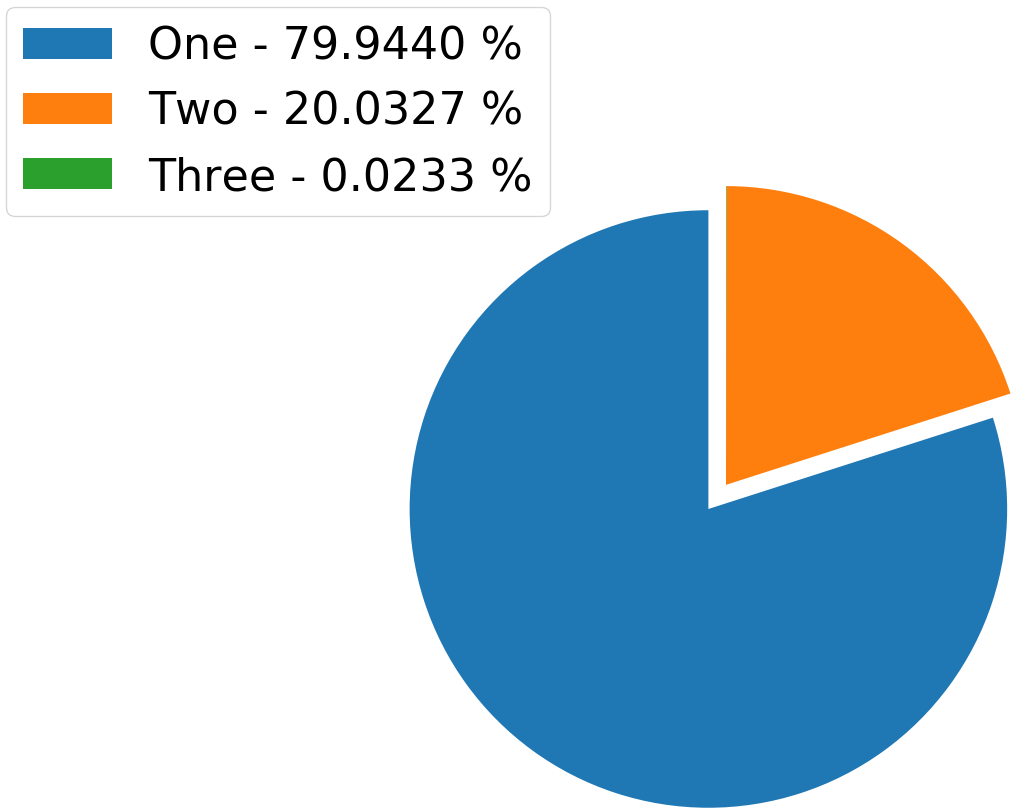
\includegraphics[width=1\linewidth]{pic/PISC_coarse.png}
    \end{minipage}
  }
  \subfigure[PISC fine]{
    \begin{minipage}[t]{0.45\linewidth}
      \centering
      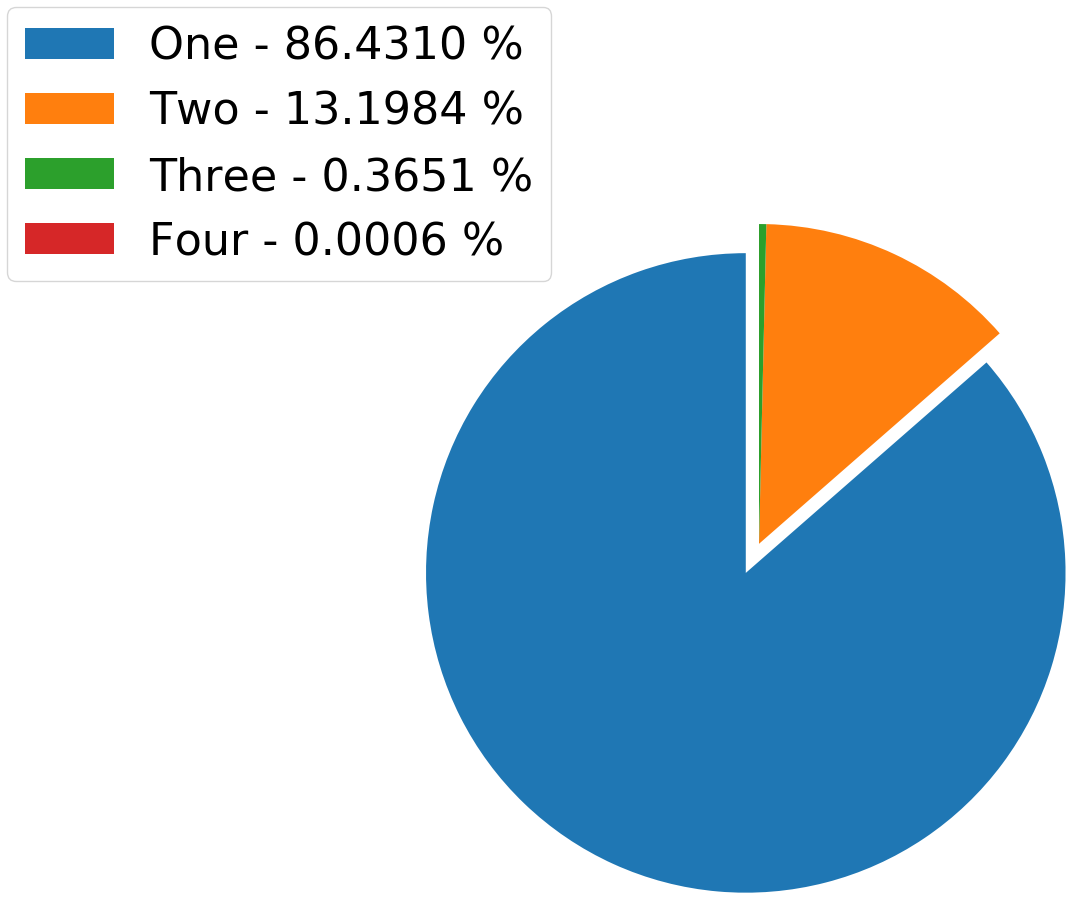
\includegraphics[width=1\linewidth]{pic/PISC_fine.png}
    \end{minipage}
  }
  \subfigure[PIPA-relation 16]{
    \begin{minipage}[t]{0.45\linewidth}
      \centering
      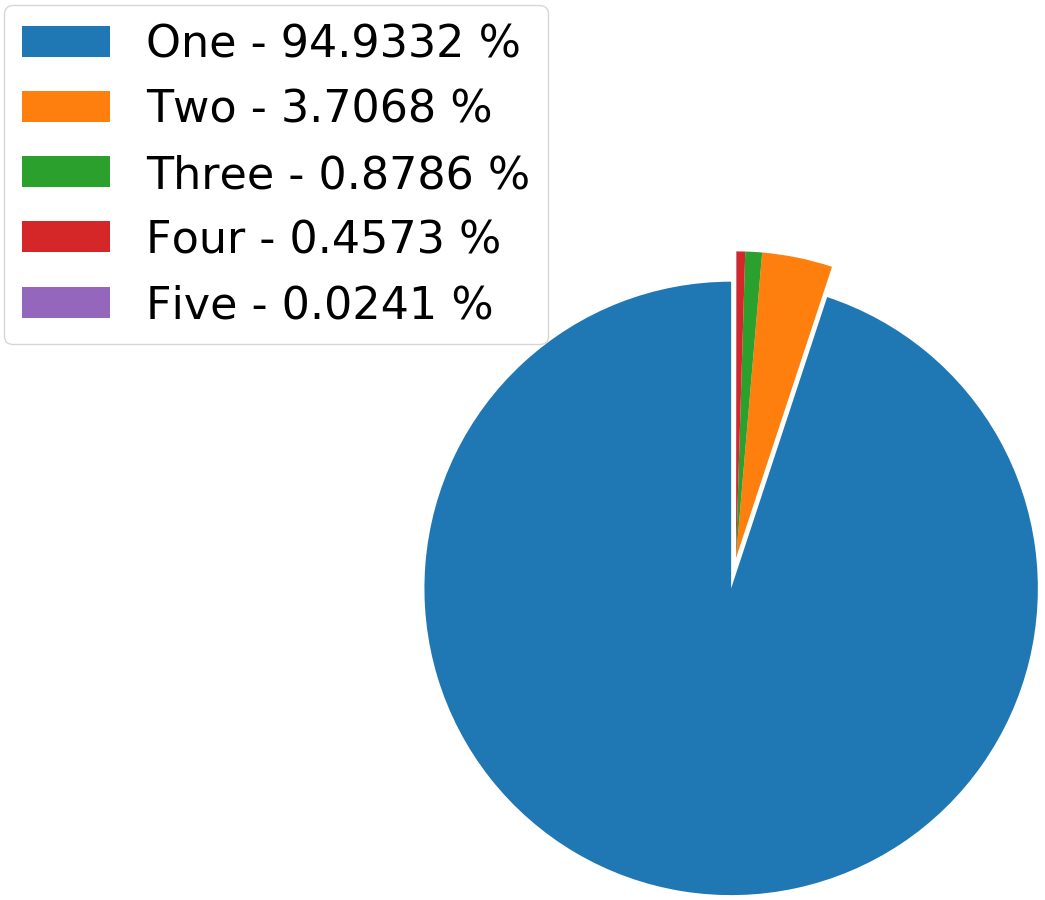
\includegraphics[width=1\linewidth]{pic/PIPA_fine.png}
    \end{minipage}
  }
  % \includegraphics[width=0.8\linewidth]{name.ext}
  \caption{Social relaion categories per image on PISC and PIPA-relation.}
  \label{fig:dataset_analysis}
\end{figure}

In this section we gave an analysis on PISC and PIPA-relation. Here we only used its train set and test set for statistic. As shown in Figure \ref{fig:dataset_analysis}, we first calculated the social relation categories of each image, and found almost all images have only one social relation category, and the other half have two categories. For example, on PISC, approximately 79.944\% of images have only one coarse category, while 20.0327\% images have two coarse one.

\subsection{Comparisons with State-of-the-Art Methods}

We compare our proposed model with existing state-of-the-art methods on both PISC and PIPA-Relation datasets.Formally, the compared methods are as followed:
\subsubsection{Performance on the PISC dataset}
{\bf UnionCNN}  Following \cite{DBLP:conf/eccv/LuKBL16}, it generates a single CNN model to predicate relations. In this task, we also feeds the union region of person pair to s single CNN for classification.\\
{\bf Pair CNN}\cite{DBLP:conf/iccv/LiWZK17} consists of two equivalent CNNs with shared weights to extracted features for image for two individuals.\\
{\bf Pair CNN + BBox + Union}\cite{DBLP:conf/iccv/LiWZK17} incorporates spatial location information of two bounding box that based the previous pair CNN and Union CNN.\\
{\bf Dual-glance}\cite{DBLP:conf/iccv/LiWZK17} implements coarse and fine prediction which includes three and six relationships. Dual-glance employing pair CNN + BBox + BBox + Union and utilized surrounding region proposal to refine the prediction.\\
{\bf GRM}\cite{DBLP:conf/ijcai/WangCRYCL18} propse a graph reasoning model that unifies the frequence of co-concurrences of each relationship-object pair to facilitate social relation.
Similar to the model of GRM, we also adopt the per-class recall and mean average precision(mMP) to evaluate our model. The experiments data are reported in Table 1. First, both Pair CNN + BBox + Union, Pair CNN + BBox + Global, Dual-glance are incur extra Faster-RCNN\cite{DBLP:conf/nips/RenHGS15} to extract the local contextual cues(object proposal). GRM utilized the object proposal to construct a semantic-aware  knowledge graph to reason about the social relationship. It is notable that both of them incur extra detection annotations that contains noisies. dasdasdasd

\subsubsection{Performance on the PIPA-Relation dataset}
On this dataset, we also compare our proposed model with the existing Two stream CNN\cite{DBLP:conf/cvpr/SunSF17},Dual-glance\cite{DBLP:conf/iccv/LiWZK17} and GRM\cite{DBLP:conf/ijcai/WangCRYCL18}.Two stream CNN takes 

\subsection{Experiment Results}

\begin{table*}[htpb]
  \centering
  \caption{Recall-per-class and mean average precision (mAP) evaluating our PRN model and previous methods on PISC (in \%).}
  \label{tab:pisc_table}
  \begin{tabular}{c|p{0.5cm}<{\centering}|p{0.5cm}<{\centering}|p{0.5cm}<{\centering}|p{0.5cm}<{\centering}||p{0.5cm}<{\centering}|p{0.5cm}<{\centering}|p{0.5cm}<{\centering}|p{0.5cm}<{\centering}|p{0.5cm}<{\centering}|p{0.5cm}<{\centering}|p{0.5cm}<{\centering}}
    \hline
    \multirow{2}{*}{Methods} & \multicolumn{4}{c|}{Coarse relationships} & \multicolumn{7}{|c}{Fine relationships} \\
    \cline{2-12}
    ~ & \rotatebox[origin=l]{90}{Intimate} & \rotatebox[origin=l]{90}{Non-Intimate} & \rotatebox[origin=l]{90}{No Relation} & \rotatebox[origin=l]{90}{mAP} & \rotatebox[origin=l]{90}{Friends} & \rotatebox[origin=l]{90}{Family} & \rotatebox[origin=l]{90}{Couple} & \rotatebox[origin=l]{90}{Professional} & \rotatebox[origin=l]{90}{Commerical} & \rotatebox[origin=l]{90}{No Relation} & \rotatebox[origin=l]{90}{mAP} \\
    \hline\hline
    Union CNN \cite{DBLP:conf/eccv/LuKBL16} & 72.1 & 81.8 & 19.2 & 58.4 & 29.9 & 58.5 & 70.7 & 55.4 & 43.0 & 19.6 & 43.5 \\
    Pair CNN \cite{DBLP:conf/iccv/LiWZK17} & 70.3 & 80.5 & 38.8 & 65.1 & 30.2 & 59.1 & 69.4 & 57.5 & 41.9 & 34.2 & 48.2 \\
    Pair CNN + BBox + Union \cite{DBLP:conf/iccv/LiWZK17} & 71.1 & 81.2 & 57.9 & 72.2 & 32.5 & 62.1 & 73.9 & 61.4 & 46.0 & 52.1 & 56.9 \\
    Pair CNN + BBox + Global \cite{DBLP:conf/iccv/LiWZK17} & 70.5 & 80.0 & 53.7 & 70.5 & 32.2 & 61.7 & 72.6 & 60.8 & 44.3 & 51.0 & 54.6 \\
    Dual-glance \cite{DBLP:conf/iccv/LiWZK17} & 73.1 & 84.2 & 59.6 & 79.7 & 35.4 & 68.1 & 76.3 & 70.3 & 57.6 & 60.9 & 63.2 \\
    GRM \cite{DBLP:conf/ijcai/WangCRYCL18} & 81.7 & 73.4 & 65.5 & 82.8 & 59.6 & 64.4 & 58.6 & 76.6 & 39.5 & 67.7 & 68.7 \\
    \hline
    Ours & & & & & & & & & & & \\
    \hline
  \end{tabular}
\end{table*}

\begin{table}[htpb]
  \centering
  \caption{Accuracy (in \%) evaluating our PRN model and previous methods on PIPA-relation.}
  \label{tab:pipa_table}
  \begin{tabular}{c|c}
    \hline
    Methods & accuracy \\
    \hline\hline
    Two stream CNN \cite{DBLP:conf/cvpr/ZhangPTFB15} & 57.2 \\
    Dual-Glance \cite{DBLP:conf/iccv/LiWZK17} & 59.6 \\
    GRM \cite{DBLP:conf/ijcai/WangCRYCL18} & 62.3 \\
    \hline
    Ours & \\
    \hline
  \end{tabular}
\end{table}

\subsection{Experiment Analysis}
\subsection{Ablation Study}
\subsection{Case Study}

\section{Conclusion}
This part will be written by {\bf liangjinrui}.

\newpage
%% The file named.bst is a bibliography style file for BibTeX 0.99c
\bibliographystyle{named}
\bibliography{ijcai19}

\end{document}
